\section{Data handling and design choices of the models}
This chapter presents how the pre-processed data is loaded and prepared for training of the models in Python, as well as the different architectures of the models, and features related to their implementation. Three separate models have been made fitting to each of the data representations described in section \ref{sec:prepros}. 

\subsection{Data handling in python}
The pre-processed data is loaded from a \textit{.mat} file into python.
Data within the file is pre-shuffled and split into a training and test subsets, as described in \autoref{sec:pre-process}. 
% The reason for shuffle the data is that improves generalisation through randomization.
In Python the training subset is further divided into a training and validation set. 
The training set is used to find the "optimal" weights with the backpropagation algorithm \citep{Bengio2012}. In this project, training set makes the biggest percentage amount of the data up to 75\%.
The validation set is used for estimating the generalization error of the model, and to examine how adjustments to hyperparameters effect the model performance \citep{Duda2000}. Hyperparameters often define many different values that can be adjusted, to control the behavior of the algorithm, to which some parameters may affect the runtime and computational cost when training the model \citep{Goodfellow2016}.The validation set makes up 10\% of the available data for the different models.
The test subset will only be used to evaluate the generalization of the model, and therefore will not contain data that has been used during the training \citep{Duda2000}.
By keeping the test subset separate it will act as new unseen data, for the model. It contains 15\% of the data.

For the binary, and combined pain map representation, the images were reshaped from a row vector, back into a matrix to retain their 2D structure. 

Furthermore the classification labels were one-hot encoded, so they were compatible to the number of outputs in the models. This is a result of the loss function \textit{categorical\_crossentropy} used for the models, that tries to reduce loss between the categories. This demands that the class label has the same dimension as the number of outputs in the model \citep{Chollet2015}.    

\subsection{Optimization techniques}
To try to reduce overfitting and improve generalization of the neural network different techniques are applied network models.

One method used to automatically chose hyperparameters is used, and is known as grid search \citep{Goodfellow2016}. By using this method a listing of different hyperparameters were tested on a model, that allowed for choosing the parameter that give the highest improvements in performance in relation to the validation loss and accuracy.  

Grid search is mainly practical when there are only a few hyperparameters that needs to be tested, because of the exponentially computational cost follows \citep{Goodfellow2016}.   

\subsubsection{Optimizer used for the models}
The Adam has been implemented in the three models, based on the findings of comparing it to the performance results with stochastic gradient descent optimizer. Adams optimizers showed a higher accuracy and significant higher training speed. Comparison results can be seen in \ref{picture from CMD}
% written in \autoref{deeplearning}.

\subsubsection{Kernel-initializer}
Kernel-initialization was performed, since it affects the performance of the model.
A grid search of kernel-initializer using \textit{uniform}, \textit{lecun\_uniform}, \textit{normal}, \textit{glorot\_normal} and \textit{glorot\_uniform} were tested and results revealed that \textit{glorot\_normal} performed the best by 3,2 \% compared to the second best. Results can be seen in \ref{picture from CMD}
% See image - kernal_init.png 

\subsubsection{Learning rate}
In order to determine the most optimal \textit{learning\_rate} for the adam optimizer a several different values were tested. To fit the model this parameter was set to \textit{0,0001} (lower than default value) meaning that the convergence of gradient descent is reached slower but with more accurate \textit{minima}. It showed the 

\subsubsection{Batch training}
Initial experimentation of the batch size showed little flexibility, because of the available computation power for training of the model. The batch size could not exceed a value of four, by reason of the relative high image resolution (912 x 2315). As a result of this it was chosen reduce the resolution (233 x 251). Resizing of the images, are described in \ref{sec:prepros}.

Furthermore, the grid search of batch parameters were performed with values of 5, 10, 15, 20, and the highest accuracy with the value 5 were chosen

\subsubsection{Cross-validation}
Because the amount of data for this project is limited it is chosen to implement m-fold cross validation, where the training data is divided into \textit{m} number of subsets. Each of the subsets can function a either a validation set or as a part of a training set e.g. if a classifier is trained \textit{m} times, then each time a different subset will be used as a validation set, and the rest is used for training. \citep{Duda2000}
Because of the property of cross validation, it can be used as a way of investigate a general accuracy since all data is included during training, but may not be beneficial for every kind of problem. \citep{Duda2000}

\subsubsection{Dropout}
Dropout is implemented in the models due to the benefits described in section \ref{sec:dropout}. The dropout is only used within the hidden fully-connected layers, where it’s defined to randomly drop 50 \% of the nodes.

\subsubsection{Activation function}
ReLu activation function is used as controlling unit for nodes activation. It defines when the node is considered as active. In the model ReLu is  implemented in convolutional and fully-connected layers.

Sigmoid is implemented only in the output layer, because it 

It has something to with the fact that the output layer performs the classification and needs sigmoid is more sutible for this task then ReLu...   

%Additional info that need to be placed somewhere.% There are simple methods that can be used to improve performance and training speed. Scaling of the input and giving an initial weight \citep{Duda2000}
%Maybe the grid test support this as well, and maybe also something about computation power.and the sigmoid for the output layer. 

\subsection{Training of the networks}
Supervised learning is used for training in all the models. The generic input for all of the model is gender, along with the different image representation, which are presented in /ref{to data}. These inputs trained and then compared against their respective category label.  WE CAN MENTION HERE THE TYPES OF DATA AND TYPES OF MODELS IF THEY ARE NOT PRESENTED LATER

%TEMP CRAP THAT NEEDS TO BE PLACED ELSEWHERE
Temp-placehoder:
The process of making the neural network model has been a trial and error process, because there is not an actual “cookbook” for developing NN (This statement is from a not vaild source, but so far it’s the only one that i have found.) \citep{Goodfellow2016}

\section{Vector image model}\label{sec:SimpleRepModel}
The architecture for this model only contains fully connected layer, since the data representation only contains 21 element vector that reflects the active pain regions and gender as described in \autoref{LinetteAndBirgithe}. It is evaluated that there would not be any gains in making the model more complex e.g. adding of convolution, based on the information available from vector, since the level of detail in relation to morphology is very simple.
The architecture of the model is illustrated in \autoref{fig:simpleModel}.

\begin{figure} [H]
\centering
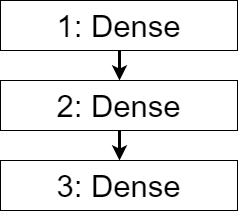
\includegraphics[width=0.3\textwidth]{figures/simpleModel}
\caption{Arcitechture of the neural network using knee region representation.}
\label{fig:simpleModel} 
\end{figure}

The model consists of three layers, where the input and output layer..(WE ADD MORE)

\section{Raw binary representation model}\label{sec:BinaryRepModel}
The architecture of this model is based on the typical structure of a convolutional network, where the first layers alternate between convolutional layers and max pooling layers \citep{LeCun2015}. This defines the first part of the model. The following layers consists of three fully connected layers, and output layer, and defined the second part of the model. An overview of the architecture is shown in \autoref{fig:binaryRepModel}. 
Convolution layer are implemented for this pain map representation, because of their ability to extract morphology features from images, as written in \autoref{CONVOLUTION}

\begin{figure} [H]
\centering
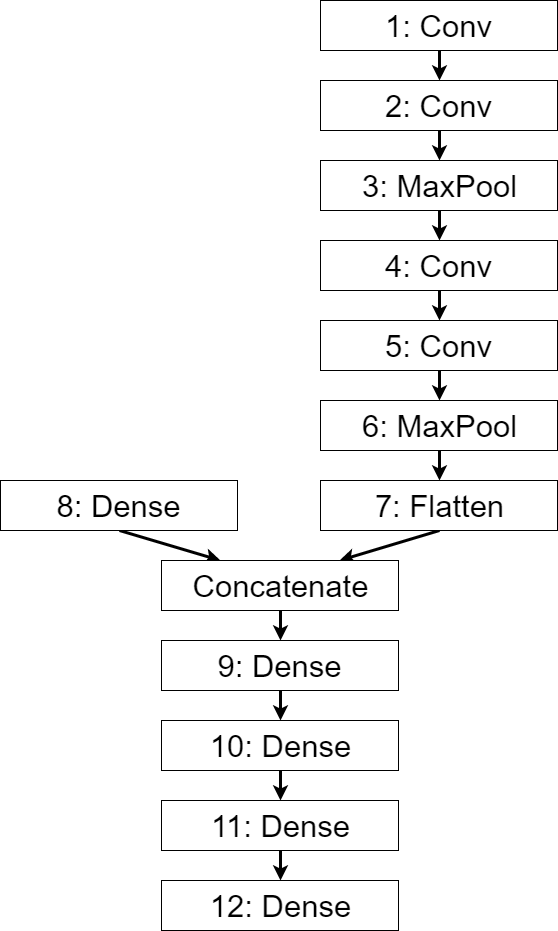
\includegraphics[width=0.6\textwidth]{figures/binaryRepModel}
\caption{Architecture for the neural network model using binary pain map representation. REMEMBER TO INCLUDE THE INPUT IN THE FIGURE}
\label{fig:binaryRepModel} 
\end{figure}

\noindent
Rather then feeding both pain map representation and gender into the same input layer, they are separated and used as input at two different locations.
The binary pain map representation works as input in first part of the model, where the input layer is a convolution layer.
This layer is setup to receive a input shape to that of the dimension of the pain map, that is defined during re-scaleing of the pain maps in \ref{LINETTE&BIRGITHE}.
Gender works as secondary input in the second section of the model, along with the pain maps features extracted through the convolution layers. Before the pain maps features reach the fully connected part of the network it is flattened from a matrix to a single row in order to merge the features with gender.
The merged data passes the fully connected layers and reaches the output layer where it is given a percentage value according to which class it fits the most.
The second part of the model resembles the simple representation model, described in \ref{sec:SimpleRepModel}

\noindent
THIS NEEDS TO BE REWRITTEN: The reason for separating gender and binary images is given as separate inputs is because of that there is no benefit in feeding gender through several convolutional layers, since these layer are use for looking at the shapes of the pain. 
\noindent
The reason for using gender as input this far into the model, is a result of the way that convolution works

\section{Combined representation model}\label{sec:CombinedRepModel}
The architecture of this model is nearly identical to that of the binary representation model as described in \ref{sec:BinaryRepModel}.
The main difference can only be seen in the input layer for the pain map representation, where the input shape is altered to contain 20 layers per pain maps instead of one.
This is the result of the one hot encoding done to the images as described in \autoref{sec:combined}.